\begin{frame}
    \titlepage
\end{frame}

\section{last time}

\begin{frame}{last time}
    \begin{itemize}
    \item various kinds of \myemph{armored} malware
        \begin{itemize}
        \item malware that evades analysis
        \end{itemize}
    \end{itemize}
\end{frame}

\begin{frame}{logistics: LEX homework}
    \begin{itemize}
    \item detect push ret pattern
    \item using flex
    \vspace{.5cm}
    \item probably easier than TRICKY
    \end{itemize}
\end{frame}

\begin{frame}{upcoming exam}
    \begin{itemize}
    \item next Wednesday
    \item review next Monday --- come with questions
    \end{itemize}
\end{frame}

\begin{frame}{armored viruses}
    \begin{itemize}
    \item ``encrypted'' malware
        \begin{itemize}
        \item not strong encryption --- key is there!
        \end{itemize}
    \item self-changing viruses:
    \begin{tikzpicture}
    \begin{scope}[start chain=going right,node distance=5mm]
    \tikzset{
        every node/.style={font=\small,join,on chain},
        every join/.style={thick,Latex-Latex},
    }
    \node {encrypted};
    \node {oligiomorphic};
    \node {polymorphic};
    \node {metamorphic};
    \end{scope}
    \end{tikzpicture}
    \item other anti-analysis techniques:   
        \begin{itemize}
        \item antigoat
        \item antiemulation
        \item antidebugging
        \end{itemize}
    \end{itemize}
\end{frame}

\begin{frame}{this time}
    \begin{itemize}
    \item finish up anti-debugging
    \item ``\myemph{tunnelling} viruses''
        \begin{itemize}
        \item evade \myemph{behavior-based} detection
        \end{itemize}
    \item memory residence
    \item Nasi article on evading 2014 antivirus
    \vspace{.5cm}
    \item (if time) new topic: exploits and stack-smashing
    \end{itemize}
\end{frame}

\section{antidebugging}

% FIXME: move to index slide?
\begin{frame}<2>[label=moreantianti]{antiantivirus} 
    \begin{itemize}
    \item last time:
        \begin{itemize}
        \item break disassemblers --- with packers
        \item break VMs/emulators
        \end{itemize}
    \item \myemph<2>{break debuggers}
        \begin{itemize}
        \item make analysis harder
        \end{itemize}
    \item \myemph<3>{break antivirus software itself}
        \begin{itemize}
        \item ``retrovirus''
        \end{itemize}
    \end{itemize}
\end{frame}

\begin{frame}<1>[label=debuggerThings]{diversion: debuggers}
    \begin{itemize}
    \item we'll care about two pieces of functionality:
    \vspace{.5cm}
    \item \myemph<2>{breakpoints}
        \begin{itemize}
        \item debugger gets control when certain code is reached
        \end{itemize}
    \item \myemph<3>{single-step}
        \begin{itemize}
        \item debugger gets control after a single instruction runs
        \end{itemize}
    \end{itemize}
\end{frame}

\subsection{breakpoints}

\againframe<2>{debuggerThings}

\begin{frame}[fragile,label=implBreak]{implementing breakpoints}
\lstset{language=myasm,style=small}
\begin{itemize}
    \item idea: change
\begin{lstlisting}
movq %rax, %rdx
addq %rbx, %rdx // BREAKPOINT HERE
subq 0(%rsp), %r8
...
\end{lstlisting}
into
\begin{lstlisting}
movq %rax, %rdx
jmp debugger_code 
subq 0(%rsp), %r8
...
\end{lstlisting}
    \item<2> problem: {\tt jmp} might be bigger than {\tt addq}?
\end{itemize}
\end{frame}

\begin{frame}[fragile,label=implBreak2]{int 3}
    \begin{itemize}
    \item x86 breakpoint instruction: {\tt \textbf{int} 3}
        \begin{itemize}
        \item Why 3? fourth entry in table of handlers
        \end{itemize}
    \item \myemph{one byte} instruction encoding: {\tt CC}
    \item debugger \myemph{modifies code to insert breakpoint}
        \begin{itemize}
        \item has copy of original somewhere
        \end{itemize}
    \item invokes handler setup by OS
        \begin{itemize}
        \item debugger can ask OS to be run by handler
        \item or changes pointer to handler directly on old OSes
        \end{itemize}
    \end{itemize}
\end{frame}

\begin{frame}{int 3 handler}
    \begin{itemize}
    \item kind of exception handler
        \begin{itemize}
        \item recall: exception handler = way for CPU to run OS code
        \end{itemize}
    \item x86 CPU saves registers, PC for debugger
    \item x86 CPU has easy to way to resume debugged code from handler
    \end{itemize}
\end{frame}

\begin{frame}[fragile,label=int3Check]{detecting int 3 directly (1)}
\lstset{language=myasm,style=small}
\begin{itemize}
    \item checksum running code
\end{itemize}
\begin{lstlisting}
mycode:
    ...
    movq $0, %rbx
    movq $mycode, %rax
loop:
    addq (%rax), %rbx
    addq $8, %rax
    cmpq $endcode, %rax
    jl loop
    cmpq %rbx, $EXPECTED_VALUE
    jne debugger_found
    ...
endcode:
\end{lstlisting}
\end{frame}

\begin{frame}[fragile,label=int3OSAPI]{detecting int 3 directly (2)}
\lstset{language=C,style=small}
\begin{itemize}
    \item query the ``handler'' for int 3
        \begin{itemize}
        \item old OSs only; today: cannot set directly
        \end{itemize}
    \item modern OSs: ask if there's a debugger attached
    \item \ldots or try to attach as debugger yourself
        \begin{itemize}
        \item doesn't work --- debugger present, probably
        \item does work --- broke any debugger?
        \end{itemize}
\end{itemize}
\begin{lstlisting}
 // Windows API function!
if (IsDebuggerPresent()) {
\end{lstlisting}
\end{frame}

\begin{frame}{modern debuggers}
    \begin{itemize}
    \item {\tt int 3} is the oldest x86 debugging mechanism
    \item modern x86: 4 ``breakpoint'' registers (\myemph{DR0--DR3})
        \begin{itemize}
        \item contain address of program instructions
        \item need more than 4? sorry
        \end{itemize}
    \item processor triggers exception when address reached
        \begin{itemize}
        \item 4 extra registers + comparators in CPU?
        \end{itemize}
    \item flag to invoke debugger if debugging registers used
        \begin{itemize}
        \item enables nested debugging
        \end{itemize}
    \end{itemize}
\end{frame}

\subsection{single stepping}

\againframe<3>{debuggerThings}

\begin{frame}[fragile,label=implSingleStep]{implementing single-stepping (1)}
\lstset{language=myasm,style=small}
\begin{itemize}
\item set a breakpoint on the following instruction? kinda works
\begin{lstlisting}
movq %rax, %rdx
addq %rbx, %rdx // <-- STOPPED HERE
subq 0(%rsp), %r8 // <-- SINGLE STEP TO HERE
subq 8(%rsp), %r8
\end{lstlisting}
transformed to
\begin{lstlisting}
movq %rax, %rdx
addq %rbx, %rdx // <-- STOPPED HERE
int 3 // <-- SINGLE STEP TO HERE
subq 8(%rsp), %r8
\end{lstlisting}
then {\tt jmp} to {\tt addq}
\end{itemize}
\end{frame}

\begin{frame}[fragile,label=implSingleStep2]{implementing single-stepping (2)}
\lstset{language=myasm,style=small}
\begin{itemize}
    \item problem: what about flow control?
\end{itemize}
\begin{lstlisting}
jmpq *0x1234(%rax,%rbx,8) // <-- STOPPED HERE
\end{lstlisting}
or
\begin{lstlisting}
retq
\end{lstlisting}
or
\begin{lstlisting}

\end{lstlisting}
\end{frame}

\begin{frame}[fragile,label=implSingleStepB]{implementing single-stepping (3)}
\lstset{language=myasm,style=small}
    \begin{itemize}
    \item typically \myemph{hardware support} for single stepping
    \item x86:{\tt int 1} handler (second entry in table)
    \item x86: {\tt TF} flag: execute handler after every instruction
    \item \ldots except during handler (whew!)
    \end{itemize}
\end{frame}

\begin{frame}[fragile,label=defeatSingleStep]{defeating single-stepping}
    \begin{itemize}
    \item try to install your own {\tt int 1} handler
        \begin{itemize}
        \item (if OS allows)
        \end{itemize}
    \item try to clear TF?
        \begin{itemize}
        \item would take effect on \myemph{following} instruction
        \item \ldots if debugger doesn't reset it
        \end{itemize}
    \end{itemize}
\end{frame}

\subsection{misc. antidebugging}

\begin{frame}[fragile,label=unstealthyDebuggers]{unstealthy debuggers}
    \begin{itemize}
    \item is a debugger installed?
        \begin{itemize}
        \item unlikely on Windows, maybe ignore those machines
        \end{itemize}
    \item is a debugger process running (don't check if it's tracing you)
    \item \ldots
    \end{itemize}
\end{frame}

\begin{frame}{confusing debuggers}
    \begin{itemize}
    \item \myemph<2>{``broken'' executable formats}
        \begin{itemize}
        \item e.g., recall ELF: segments and sections
        \item corrupt sections --- program still works
        \item overlapping segments/sections --- program still works
        \item what does the loader really use??
        \end{itemize}
    \item \myemph<3>{``broken'' machine code}
        \begin{itemize}
        \item insert ``junk'' bytes to break disassembly
        \item skip over junk with jump
        \end{itemize}
    \item \myemph<4>{use the stack pointer not for the stack}
        \begin{itemize}
        \item stack trace?
        \end{itemize}
    \end{itemize}
    \begin{tikzpicture}[overlay,remember picture]
        \begin{visibleenv}<2>
            \node[draw=red,fill=white,align=center] at (current page.center) {
                recall anti-virus heuristics looking for this \\
                (though brokness probably not on purpose?)
            };
        \end{visibleenv}
        \begin{visibleenv}<3>
            \node[draw=red,fill=white] at (current page.center) {
                ``encrypted'' code sophisticated version of this 
            };
        \end{visibleenv}
    \end{tikzpicture}
\end{frame}

\section{retroviruses, etc.}

\againframe<3>{moreantianti}

\begin{frame}{terminology}
    \begin{itemize}
    \item \textit{semistealth}/\textit{stealth} --- hide from system
    \item \textit{tunneling virus} --- evades behavior-blocking
        \begin{itemize}
        \item e.g. detection of modifying system files
        \end{itemize}
    \item \textit{retrovirus} --- directly attacks/disables antivirus software
    \end{itemize}
\end{frame}

\begin{frame}{attacking antivirus (1)}
    \begin{itemize}
    \item how does antivirus software scan new files?
    \item how does antivirus software detect bad behavior?
        \begin{itemize}
        \item register handlers with OS/applications --- new files, etc.
        \end{itemize}
    \end{itemize}
\end{frame}

\begin{frame}[label=hookingReason]{hooking and malware}
    \begin{itemize}
    \item \myemph{hooking} --- getting a `hook' into (OS) operations
        \begin{itemize}
        \item e.g. creating new files, opening file
        \item monitoring or changing/stopping behavior
        \end{itemize}
    \item used by antivirus and malware:
    \vspace{.5cm}
    \item \myemph{stealth} virus --- hide virus program from normal I/O, etc.
    \item \myemph{tunneling} virus --- skip over antivirus's hook
    \item \myemph{retrovirus} --- break antivirus's hook
    \end{itemize}
\end{frame}

\subsection{stealth}

\begin{frame}[fragile,label=stealth]{stealth}
\lstset{language=C,style=small}
\begin{lstlisting}
/* in virus: */
int OpenFile(const char *filename, ...) {
    if (strcmp(filename, "infected.exe") == 0) {
        return RealOpenFile("clean.exe", ...);
    } else {
        return RealOpenFile(filename, ...);
    }
}
\end{lstlisting}
\end{frame}

\begin{frame}{stealth ideas}
    \begin{itemize}
    \item override ``get file modification time'' (infected files)
    \item override ``get files in directory'' (infected files)
    \item override ``read file'' (infected files)
        \begin{itemize}
        \item but not ``execute file''
        \end{itemize}
    \item override ``get running processes'' 
    \end{itemize}
\end{frame}

\subsection{tunneling}

\begin{frame}{tunneling ideas}
    \begin{itemize}
    \item use the ``real'' write/etc. function
        \begin{itemize}
        \item not wrapper from antivirus software
        \end{itemize}
    \item find write/etc. function antivirus software ``forgot'' to hook
    \end{itemize}
\end{frame}

\subsection{retrovirus}

\begin{frame}{retrovirus ideas}
    \begin{itemize}
    \item empty antivirus signature list
    \item kill antivirus process, remove ``hooks''
    \item delete antivirus software, replace with dummy executable
    \item \ldots
    \end{itemize}
\end{frame}

\subsection{hooking mechanisms}

\begin{frame}<1>[label=hookingList]{hooking mechanisms}
    \begin{itemize}
    \item hooking --- getting a `hook' to run on (OS) operations
        \begin{itemize}
        \item e.g. creating new files
        \end{itemize}
    \item ideal mechanism: \myemph<2>{OS support}
    \item less ideal mechanism: \myemph<3>{change library loading}
        \begin{itemize}
        \item e.g. replace `open', `fopen', etc. in libraries
        \end{itemize}
    \item less ideal mechanism: \myemph<4>{replace OS exception} (system call) handlers
        \begin{itemize}
        \item very OS version dependent
        \end{itemize} 
    \end{itemize}
\end{frame}

\againframe<2>{hookingList}

\begin{frame}
\begin{centering}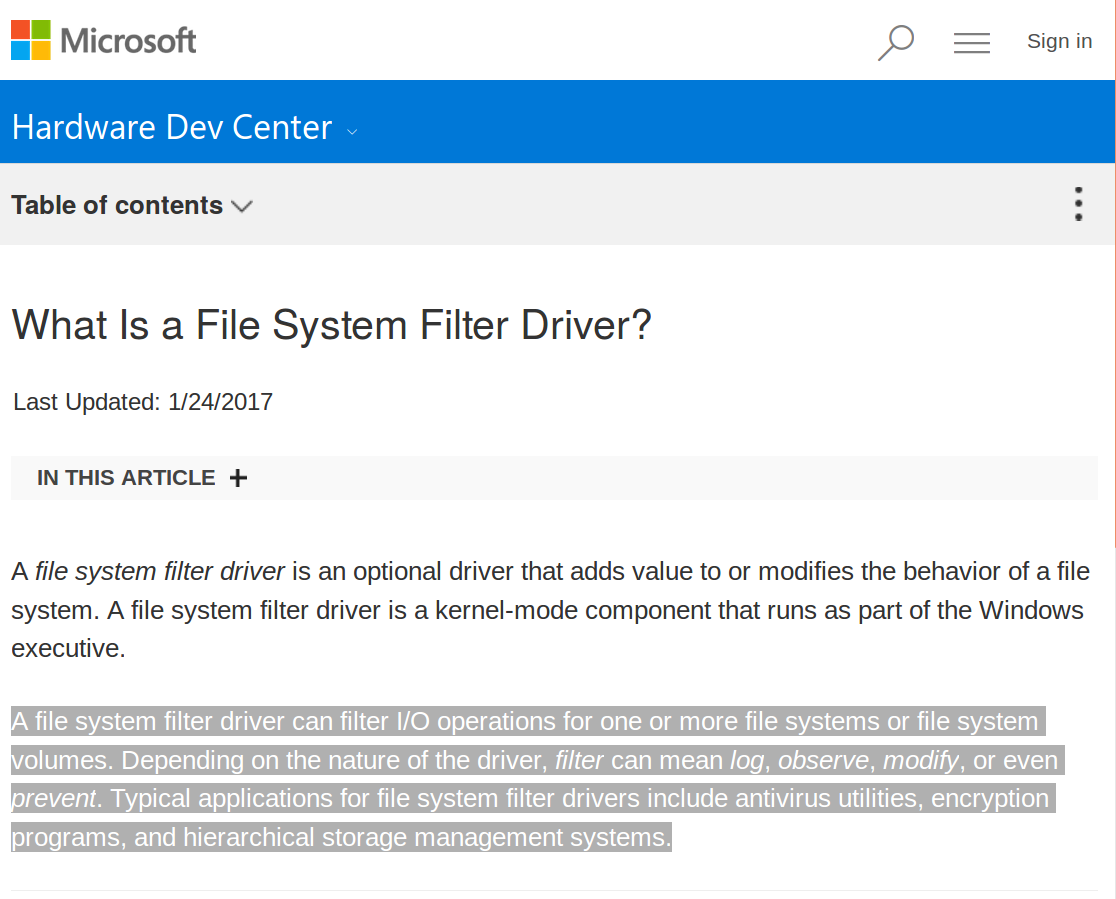
\includegraphics[height=0.9\textheight]{filter-driver}\end{centering}
\end{frame}

\begin{frame}{debugging mechanisms}
    \begin{itemize}
    \item debuggers can stop program at system calls, etc.
    \item another form of OS support, typically
    \item Linux interface: {\tt ptrace}
        \begin{itemize}
        \item has ``run program until any system call'' mode
        \item and (recently) `` run program until specific system call'' mode
        \end{itemize}
    \end{itemize}
\end{frame}

\againframe<3>{hookingList}

\begin{frame}{changing library loading}
\begin{itemize}
    \item e.g. install new library --- or edit loader, but \ldots
    \vspace{.5cm}
    \item not everything uses library functions
    \item what if your wrapper doesn't work exactly the same?
        \begin{itemize}
        \item ``anti-virus breaks my program''
        \end{itemize}
    \end{itemize}
\end{frame}

\againframe<4>{hookingList}

\begin{frame}{changing exception handlers?}
    \begin{itemize}
    \item mechanism on DOS
    \item track what old exception handler does
    \item ``tunneling'' technique --- find the original, call it instead
    \end{itemize}
\end{frame}

\begin{frame}{other holes in behavior blocking}
    \begin{itemize}
    \item if in library: don't use library function
        \begin{itemize}
        \item e.g. copy of ``clean'' library
        \item e.g. statically linked
        \end{itemize}
    \item generally: multiple ways to do things?
        \begin{itemize}
        \item like VM problem: was something missed?
        \end{itemize}
    \vspace{.5cm}
    \item e.g.. file modifications blocked?
    \item just acccess the disk directly
    \end{itemize}
\end{frame}

\subsection{misc. retrovirus mechanisms}

\begin{frame}{attacking antivirus (2)}
    \begin{itemize}
    \item mechanisms other than hooking
    \item just directly modify it
        \begin{itemize}
        \item example: IDEA.6155 modifies database of scanned files
        \end{itemize}
    \item preserve checksums
        \begin{itemize}
        \item example: HybrisF preserved CRC32 checksums of infected files
        \item some AV software won't scan again
        \item solution: use cryptographically secure hashes instead
        \end{itemize}
    \end{itemize}
\end{frame}

\subsection{memory residence}

\begin{frame}{not just hiding/interfering}
    \begin{itemize}
    \item our model of malware --- runs when triggered
    \item reality: sometimes keep on running
        \begin{itemize}
        \item evade active detection
        \item spread to new programs/files as created/run
        \end{itemize}
    \item call \myemph{resident}
    \end{itemize}
\end{frame}

\begin{frame}{spreading in memory}
    \begin{itemize}
    \item hook to hide virus file
    \item not just hiding virus --- can propagate!
    \item example: infect any new files
    \item example: reinfect ``repaired'' files
    \end{itemize}
\end{frame}

\section{Nasi article}

\begin{frame}{Emeric Nasi article}
    \begin{itemize}
    \item Emeric Nasi, ``Bypass Antivirus Dynamic Analysis: Limitations of the AV model and how to exploit them'', 2014
    \item terminology ``FUD = Fully UnDetectable''
    \item NB --- not a peer-reviewed article
        \begin{itemize}
        \item ``non-traditional literature''
        \end{itemize}
    \item wrote programs, submitted to \myemph{VirusTotal}
        \begin{itemize}
        \item aggregator of antivirus software
        \end{itemize}
    \item looking at detection of \myemph{new malware}
    \end{itemize}
\end{frame}

\begin{frame}{techniques in Nasi that worked}
    \begin{itemize}
    \item things 2014 Antivirus VM's couldn't handle:
    \vspace{.5cm}
    \item allocate 100 MB
    \item 100M increments
    \item un/misimplemented system calls (NUMA, mutex)
    \item check executable name
    \end{itemize}
\end{frame}

% FIXME: summary


